\section{Calcul des coefficient des CIOE par moindres carrés}

% Pour calculer les coefficients, nous minimisons par moindres carrés
% \begin{itemize}
%   \item dans le cas du plan infini la différence entre l'impédance \(\hat\mZ_{ex}(k_x,k_y)\) et son approximation \(\hat\mZ_{ap}(k_x,k_y)\);
%   \item dans le cas du cylindre infini la différence entre les coefficients de Fourier \(\hat\mF_{ex}(n,k_z)\) et leurs approximations \(\hat\mF_{ap}(n,k_z)\);
%   \item dans le cas de la sphère la différence entre les coefficients de Mie \(\hat\mM_{ex}(n,m)\) et leurs approximations \(\hat\mM_{ap}(n,m)\);
% \end{itemize}
% Toutes ces quantités ont été définies aux chapitres \ref{sec:chap1} et \ref{sec:chap2}

\subsection{Expression des moindre carrés dans le cadre de l'approximation plan infini}
  Pour toutes les CIOE, on cherche à approcher la matrice \(\hat\mZ_{ex}(k_x,k_y)\) par \(\hat\mZ_{CI}(k_x,k_y)\). 

  \begin{prop}
    Soit \(N_i\) le nombre de couples \((k_x,k_y)\).
    Il existe une matrice \(\mH(CI,\hat\mZ_{ex})\) et un vecteur \(X(CI)\) de \(\CC^{N_{CI}}\) composés des coefficients de la CIOE choisie, tels que minimiser selon la norme euclidienne
    \begin{align*}
      \left\lVert \hat\mZ_{ap}(k_x,k_y)-\hat\mZ_{ex}(k_x,k_y)\right\rVert^2_{eucl} & & \text{pour tous \((k_x,k_y)\)}
    \end{align*}
    revient à minimiser selon une norme équivalente mais dépendante de la CI, la fonctionnelle
    \[ 
      F(CI) = \left\lVert  \mH(CI,\hat\mZ_{ex}) X(CI) - b(\hat\mZ_{ex}) \right\rVert^2_{CI}
    \]
    La matrice \(\mH\) a \(4N_{i}\) lignes, \(N_{CI}\) colonnes et le vecteur colonne b a \(4N_{i}\) coefficients
  \end{prop}

  \begin{proof}
    Nous démontrons ce résultat pour la \hyperlink{ci3}{CI3} où les termes \(k_0^2\) sont omis, la matrice \(\mH\) et le vecteur \(X\) des autres CIOE de déduisent facilement.

    Soient les matrices symétriques \(\hat\mLD, \hat\mLR\) telles que

    \begin{align}
      \hat\mLD(k_x,k_y) & = - \begin{bmatrix} k_x^2 & k_x k_y \\ k_x k_y & k_y^2 \end{bmatrix}
      \\
      \hat\mLR(k_x,k_y) & =  \begin{bmatrix} k_y^2 & -k_x k_y \\ -k_x k_y &  k_x^2 \end{bmatrix}
    \end{align}

    Soit \((k_{x},k_{y})\) un couple parmi ceux que l'on se donne. Pour ce couple, par définition, on a
    \begin{align}
    \left\lVert \hat\mZ_{ap}-\hat\mZ_{ex}\right\rVert^2_{eucl} &= \left\lVert \left(\mI + b_1 \hat{\mLD} - b_2 \hat{\mLR}\right)^{-1}\left(a_0\mI + a_1 \hat{\mLD} - a_2 \hat{\mLR}\right)-\hat\mZ_{ex} \right\rVert^2_{eucl}
    \\
    \intertext{Posons pour alléger les formules \(\hat{\mZ}_N = a_0\mI + a_1 \hat{\mLD} - a_2 \hat{\mLR}\) et \(\hat{\mZ}_D = \mI + b_1 \hat{\mLD} - b_2 \hat{\mLR}\)}
    \left\lVert \hat\mZ_{ap}-\hat\mZ_{ex}\right\rVert^2_{eucl} &= \left\lVert \hat{\mZ}_D^{-1}\hat\mZ_N-\hat\mZ_{ex} \right\rVert^2_{eucl}
    \\
    &= \left\lVert \hat{\mZ}_D^{-1}\left(\hat{\mZ}_N-\hat{\mZ}_D\hat\mZ_{ex}\right) \right\rVert^2_{eucl}
    \\
    \intertext{On sépare alors \(\hat{\mZ}_D\) en deux parties}
    \left\lVert \hat\mZ_{ap}-\hat\mZ_{ex}\right\rVert^2_{eucl} &= \left\lVert \hat{\mZ}_D^{-1}\left(\hat{\mZ}_N - \left(b_1 \hat{\mLD} - b_2 \hat{\mLR}\right)\hat\mZ_{ex} - \hat\mZ_{ex}\right)\right\rVert^2_{eucl}
    \intertext{On voit alors apparaitre une nouvelle norme}
    \left\lVert \hat\mZ_{ap}-\hat\mZ_{ex}\right\rVert^2_{eucl} &= \left\lVert \hat{\mZ}_N - \left(b_1 \hat{\mLD} - b_2 \hat{\mLR}\right)\hat\mZ_{ex} - \hat\mZ_{ex}\right\rVert^2_{\hat{\mZ}_D^{-1}}
  \end{align}

  On réorganise alors les matrices \(\hat{\mZ}_N,\hat{\mLD},\hat{\mLR}\) comme des vecteurs colonnes, on obtient alors une partie du système final
  \begin{align}
      \mH_{k_{x},k_{y}}(CI3,\hat\mZ) = \begin{bmatrix}
      1 & \hat{\mLD}_{11} & -\hat{\mLR}_{11} & -\left(\hat{\mLD}\hat\mZ\right)_{11} & \left(\hat{\mLR}\hat\mZ\right)_{11}
      \\
      0 & \hat{\mLD}_{12} & -\hat{\mLR}_{12} & -\left(\hat{\mLD}\hat\mZ\right)_{12} & \left(\hat{\mLR}\hat\mZ\right)_{12}
      \\
      0 & \hat{\mLD}_{21} & -\hat{\mLR}_{21} & -\left(\hat{\mLD}\hat\mZ\right)_{21} & \left(\hat{\mLR}\hat\mZ\right)_{21}
      \\
      1 & \hat{\mLD}_{22} & -\hat{\mLR}_{22} & -\left(\hat{\mLD}\hat\mZ\right)_{22} & \left(\hat{\mLR}\hat\mZ\right)_{22}
      \end{bmatrix}
  \end{align}
  \begin{align}
      b_{k_{x},k_{y}}(\hat\mZ_{ex}) = \begin{bmatrix}
      \hat\mZ_{11}
      \\
      \hat\mZ_{12}
      \\
      \hat\mZ_{21}
      \\
      \hat\mZ_{22}
      \end{bmatrix} && X = \begin{bmatrix} a_0 \\ a_1 \\ a_2 \\ b_1 \\ b_2 \end{bmatrix}
  \end{align}

  Le système final est obtenu en prenant en compte tous les couples, soit

  \begin{align}
      \mH(CI3,\hat\mZ) = 
      \begin{bmatrix}
        \mH_{k_{x1},k_{y1}}(CI3,\hat\mZ)
        \\
        \vdots
        \\
        \mH_{k_{xn},k_{yn}}(CI3,\hat\mZ)
      \end{bmatrix}
      &&  b(\hat\mZ) = 
      \begin{bmatrix}
        b_{k_{x1},k_{y1}}(\hat\mZ)
        \\
        \vdots
        \\
        b_{k_{xn},k_{yn}}(\hat\mZ)
      \end{bmatrix}
  \end{align}

  % \begin{align}
  %     \mH(CI3,\hat\mZ) = \begin{bmatrix}
  %     1 & \hat{\mLD}_{11}(k_{x1},k_{y1}) & -\hat{\mLR}_{11}(k_{x1},k_{y1}) & -\left(\hat{\mLD}(k_{x1},k_{y1})\hat\mZ(k_{x1},k_{y1})\right)_{11} & \left(\hat{\mLR}(k_{x1},k_{y1})\hat\mZ(k_{x1},k_{y1})\right)_{11}
  %     \\
  %     0 & \hat{\mLD}_{12}(k_{x1},k_{y1}) & -\hat{\mLR}_{12}(k_{x1},k_{y1}) & -\left(\hat{\mLD}(k_{x1},k_{y1})\hat\mZ(k_{x1},k_{y1})\right)_{12} & \left(\hat{\mLR}(k_{x1},k_{y1})\hat\mZ(k_{x1},k_{y1})\right)_{12}
  %     \\
  %     0 & \hat{\mLD}_{21}(k_{x1},k_{y1}) & -\hat{\mLR}_{21}(k_{x1},k_{y1}) & -\left(\hat{\mLD}(k_{x1},k_{y1})\hat\mZ(k_{x1},k_{y1})\right)_{21} & \left(\hat{\mLR}(k_{x1},k_{y1})\hat\mZ(k_{x1},k_{y1})\right)_{21}
  %     \\
  %     1 & \hat{\mLD}_{22}(k_{x1},k_{y1}) & -\hat{\mLR}_{22}(k_{x1},k_{y1}) & -\left(\hat{\mLD}(k_{x1},k_{y1})\hat\mZ(k_{x1},k_{y1})\right)_{22} & \left(\hat{\mLR}(k_{x1},k_{y1})\hat\mZ(k_{x1},k_{y1})\right)_{22}
  %     \\
  %     \vdots & \vdots & \vdots & \vdots & \vdots
  %     \\
  %     1 & \hat{\mLD}_{11}(k_{xn},k_{yn}) & -\hat{\mLR}_{11}(k_{xn},k_{yn}) & -\left(\hat{\mLD}(k_{xn},k_{yn})\hat\mZ(k_{xn},k_{yn})\right)_{11} & \left(\hat{\mLR}(k_{xn},k_{yn})\hat\mZ(k_{xn},k_{yn})\right)_{11}
  %     \\
  %     0 & \hat{\mLD}_{12}(k_{xn},k_{yn}) & -\hat{\mLR}_{12}(k_{xn},k_{yn}) & -\left(\hat{\mLD}(k_{xn},k_{yn})\hat\mZ(k_{xn},k_{yn})\right)_{12} & \left(\hat{\mLR}(k_{xn},k_{yn})\hat\mZ(k_{xn},k_{yn})\right)_{12}
  %     \\
  %     0 & \hat{\mLD}_{21}(k_{xn},k_{yn}) & -\hat{\mLR}_{21}(k_{xn},k_{yn}) & -\left(\hat{\mLD}(k_{xn},k_{yn})\hat\mZ(k_{xn},k_{yn})\right)_{21} & \left(\hat{\mLR}(k_{xn},k_{yn})\hat\mZ(k_{xn},k_{yn})\right)_{21}
  %     \\
  %     1 & \hat{\mLD}_{22}(k_{xn},k_{yn}) & -\hat{\mLR}_{22}(k_{xn},k_{yn}) & -\left(\hat{\mLD}(k_{xn},k_{yn})\hat\mZ(k_{xn},k_{yn})\right)_{22} & \left(\hat{\mLR}(k_{xn},k_{yn})\hat\mZ(k_{xn},k_{yn})\right)_{22}
  %     \end{bmatrix}
  % \end{align}
  \end{proof}

  \subsection{Existence et unicité du minimum}

    \begin{prop}
      Il existe un unique minimum si la matrice \(\conj{\mH^t}{\mH}\) est inversible
    \end{prop}

    \begin{proof}
      On remarque que la fonctionnelle \(F\) est quadratique si la matrice \(\mM=\conj{\mH^t}{\mH}\) est hermitienne définie positive. Une matrice \(A\) est hermitienne si \(\forall x, \conj{x^t}Ax \in \RR\), elle est hermitienne positive si \(\forall x, \conj{x^t}Ax \in \RR^+\) et elle est hermitienne définie positive si \(\forall x\not=0, \conj{x^t}Ax \in \RR^{+*}\).

      On remarque que par construction, notre matrice \(\mM\) est hermitienne positive. Il reste à montrer qu'elle est définie.
    \end{proof}

    \begin{prop}
      S'il existe une unique minimum \(X_{CI}^*\), celui ci vaut
      \[
        X_{CI}^* = \left(\conj{\mH_{CI}^t}{\mH_{CI}}\right)^{-1}\conj{\mH_{CI}^t}b
      \]
    \end{prop}

    \begin{proof}
      C'est une application directe de \(\tgrad{} F(CI) = 0 \), avec la propriété précédente.
    \end{proof}

    \subsubsection{Existence du minimum pour la CI4}

      \begin{prop}
        La matrice \({\mM}\) associé à la CI4 est inversible, donc définie, si et seulement s'il existe au moins 2 couples \((k_{xi},k_{yi})\) différents.
      \end{prop}

      \begin{proof}
        Soit \(t\) le vecteur de \(\left(\RR^+\right)^{N_{i}}\) tel que \(t_i = k_{xi}^2 + k_{yi}^2\). On a l'expression suivante de \({\mM}\)

        \begin{equation}
          {\mM} = \begin{bmatrix}
          2 N_{i} & -\sum_{i=1}^{N_{i}} t_i & -\sum_{i=1}^{N_{i}} t_i
          \\
          -\sum_{i=1}^{N_{i}} t_i & \sum_{i=1}^{N_{i}} t_i^2 & 0
          \\
          -\sum_{i=1}^{N_{i}} t_i & 0 & \sum_{i=1}^{N_{i}} t_i^2
          \end{bmatrix}
        \end{equation}

        Pour prouver son inversibilité, on exprime son déterminant 

        \begin{align}
          \det( {\mM}) &= 2N_{i}\left(\sum_{i=1}^{N_{i}} t_i^2\right)^2 - 2 \left( \sum_{i=1}^{N_{i}} t_i\right)^2 \left(\sum_{i=1}^{N_{i}}t_i^2\right) 
          \\
          &= 2\left(\sum_{i=1}^{N_{i}} t_i^2\right)\left(N_{i}\sum_{i=1}^{N_{i}} t_i^2 - \left( \sum_{i=1}^{N_{i}} t_i\right)^2 \right)
          \\
          \intertext{Soit \(\left<\cdot,\cdot\right>\) le produit scalaire associé à \(\RR^{N_{i}}\), alors}
          \det( {\mM}) &= 2\left<t,t\right>\left( \left<1,1\right>\left<t,t\right>- \left<t,1\right>^2\right)
        \end{align}

        Donc d'après Cauchy–Schwarz (voir \cite[\href{https://dlmf.nist.gov/1.7\#E1}{eq.~1.7.1}]{dlmf_nist_2019}), le terme de droite est non-nul pour tout \(t\) non colinéaire au vecteur dont toutes les composantes valent 1, c'est à dire n'importe quel vecteur ayant au moins deux composantes différentes.
      \end{proof}

      \subsubsection{Existence du minimum pour la CI3}

        L'introduction de \(\hat\mZ_{ex}\) dans \(\mM\) ne permet plus d'exprimer simplement le déterminant de cette dernière. Nous n'avons pas réussi à prouver que cette matrice était définie. Cependant nous avons vérifié numériquement qu'elle l'était pour tous les empilements que nous avons testés.

  \subsection{Résultats numériques sans contraintes}

      Sans contraintes, on résout le système linéaire \(\mH X = b\). 
      %Numériquement, nous avons utilisé la routine de résolution au sens des moindres carrés \href{http://www.netlib.org/lapack/explore-html/d6/d10/group__complex16_g_esolve_ga1d8089ba1e1538eb3d1ab0ebe97596c7.html}{ZGELS}.


      Dans \cite{stupfel_implementation_2015} sont introduites les CIOE
      \begin{itemize}
        \item CI01
          \begin{equation}
            \vE_t = \left(a_0\oI + a_1\frac{\LL}{k_0^2}\right)\vJ
          \end{equation}
        \item CI1
          \begin{equation}
            \left(\oI + b\frac{\LL}{k_0^2} \right)\vE_t = \left(a_0\oI + a_1\frac{\LL}{k_0^2}\right)\vJ
          \end{equation}
      \end{itemize}

      L'opérateur \(\LL\) est le laplacien tangentiel \(\lapls\) appliqué à chaque composante. Le multiplicateur de Fourier associé est la matrice
      \begin{equation}
        \hat{\mL}  = -
        \begin{bmatrix}
          k_x^2 + k_y^2 & 0
          \\
          0 & k_x^2 + k_y^2
        \end{bmatrix}
      \end{equation}

      La matrice \(\mL\) est multiple de l'identité donc la matrice \(\hat\mZ_{CI}\) associée à ces CIOE est n'approchera pas bien la matrice \(\hat{\mZ}_{ex}\). La figure \ref{fig:imp_fourier:plan:stupfel:hoibc} présente donc quelques résultats où l'on voit bien la limite de ces CIOE par rapport à la CI3.
      \begin{figure}[!hbt]
        \centering
        \tikzsetnextfilename{Z_STUPFEL_plan_hoibc.11}
\begin{tikzpicture}[scale=1]
    \begin{axis}[
            title={Polarisation TM},
            ylabel={\(|\hat{Z}(k_x,0)|\)},
            xlabel={\(k_x\slash k_0\)},
            width=0.4\textwidth,
            xmin=0,
            xmax=1,
            ymin=0.14,
            ymax=0.25,
            restrict y to domain=0:11,
            mark repeat=10,
            legend pos=outer north east
        ]
        \addplot [color=black,mark=square*] table [col sep=comma, x={s1}, y={Abs(z_ex.11)}] {csv/STUPFEL/STUPFEL.z_ex.MODE_2_TYPE_P.csv};

        \addplot [color=\ccio,mark=x] table [col sep=comma, x={s1}, y={Abs(z_ibc0.11)}] {csv/STUPFEL/STUPFEL.z_ibc.IBC_ibc0_SUC_F_MODE_2_TYPE_P.csv};

        \addplot [color=\cciou!50!black,mark=pentagon*] table [col sep=comma, x={s1}, y={Abs(z_ibc01.11)}] {csv/STUPFEL/STUPFEL.z_ibc.IBC_ibc01_SUC_F_MODE_2_TYPE_P.csv};

        \addplot [color=\cciu,mark=*] table [col sep=comma, x={s1}, y={Abs(z_ibc1.11)}] {csv/STUPFEL/STUPFEL.z_ibc.IBC_ibc1_SUC_F_MODE_2_TYPE_P.csv};

        \addplot [color=\ccit,mark=diamond*] table [col sep=comma, x={s1}, y={Abs(z_ibc3.11)}] {csv/STUPFEL/STUPFEL.z_ibc.IBC_ibc3_SUC_F_MODE_2_TYPE_P.csv};
    \end{axis}
\end{tikzpicture}
\tikzsetnextfilename{Z_STUPFEL_plan_hoibc.22}
\begin{tikzpicture}[scale=1]
    \begin{axis}[
            title={Polarisation TE},
            ylabel={},
            xlabel={\(k_x\slash k_0\)},
            width=0.4\textwidth,
            xmin=0,
            xmax=1,
            ymin=0.14,
            ymax=0.25,
            mark repeat=10,
            restrict y to domain=0:11,
            legend pos=outer north east
        ]
        \addplot [color=black,mark=square*] table [col sep=comma, x={s1}, y={Abs(z_ex.22)}] {csv/STUPFEL/STUPFEL.z_ex.MODE_2_TYPE_P.csv};
        \addlegendentry{Exact};

        \addplot [color=\ccio,mark=x] table [col sep=comma, x={s1}, y={Abs(z_ibc0.22)},color=] {csv/STUPFEL/STUPFEL.z_ibc.IBC_ibc0_SUC_F_MODE_2_TYPE_P.csv};
        \addlegendentry{CI0};

        \addplot [color=\cciou!50!black,mark=pentagon*] table [col sep=comma, x={s1}, y={Abs(z_ibc01.22)}] {csv/STUPFEL/STUPFEL.z_ibc.IBC_ibc01_SUC_F_MODE_2_TYPE_P.csv};
        \addlegendentry{CI01};

        \addplot [color=\cciu,mark=*] table [col sep=comma, x={s1}, y={Abs(z_ibc1.22)}] {csv/STUPFEL/STUPFEL.z_ibc.IBC_ibc1_SUC_F_MODE_2_TYPE_P.csv};
        \addlegendentry{CI1};

        \addplot [color=\ccit,mark=diamond*] table [col sep=comma, x={s1}, y={Abs(z_ibc3.22)}] {csv/STUPFEL/STUPFEL.z_ibc.IBC_ibc3_SUC_F_MODE_2_TYPE_P.csv};
        \addlegendentry{CI3};

    \end{axis}
\end{tikzpicture}
        \caption[CIOE sur empilement de B.~Stupfel p.~1661]{Module des coefficients diagonaux de \(\hat\mZ\) pour \(\eps = 1-i, \mu = 1, d=0.05\text{m}, f=0.2\text{GHz}\)}
        \label{fig:imp_fourier:plan:stupfel:hoibc}
      \end{figure}
      \begin{table}[!hbt]
        \centering
        \tablecoeff[0.49]{\hyperlink{ci0}{CI0}}{csv/STUPFEL/STUPFEL.IBC_ibc0_SUC_F_MODE_2_TYPE_P.coeff.txt}
        \tablecoeff[0.49]{\hyperlink{ci01}{CI01}}{csv/STUPFEL/STUPFEL.IBC_ibc01_SUC_F_MODE_2_TYPE_P.coeff.txt}

        \tablecoeff[0.49]{\hyperlink{ci1}{CI1}}{csv/STUPFEL/STUPFEL.IBC_ibc1_SUC_F_MODE_2_TYPE_P.coeff.txt}
        \tablecoeff[0.49]{\hyperlink{ci3}{CI3}}{csv/STUPFEL/STUPFEL.IBC_ibc3_SUC_F_MODE_2_TYPE_P.coeff.txt}
        \caption{Coefficients associés à la figure \ref{fig:imp_fourier:plan:stupfel:hoibc}}
        \label{tab:imp_fourier:plan:stupfel:hoibc}
      \end{table}
      
      \begin{figure}[!hbt]
        \centering
        \tikzsetnextfilename{R_STUPFEL_plan_hoibc.TM}
\begin{tikzpicture}[scale=1]
    \begin{axis}[
            title={Polarisation TM},
            ylabel={\(|\hat{R}(k_x,0)|\)},
            xlabel={\(\sin(k_x\slash k_0)^{-1}\) (deg)},
            width=0.4\textwidth,
            xmin=0,
            xmax=90,
            ymin=0.4,
            ymax=1,
            mark repeat=15,
            legend pos=outer north east
        ]
        \addplot [color=black,mark=square*] table [col sep=comma, x={theta1}, y={Abs(r_ex.11)}] {csv/STUPFEL/STUPFEL.r_ex.MODE_2_TYPE_P.csv};

        \addplot [color=blue,mark=x] table [col sep=comma, x={theta1}, y={Abs(r_ibc0.11)}] {csv/STUPFEL/STUPFEL.r_ibc.IBC_ibc0_SUC_F_MODE_2_TYPE_P.csv};

        \addplot [color=green!50!black,mark=pentagon*] table [col sep=comma, x={theta1}, y={Abs(r_ibc01.11)}] {csv/STUPFEL/STUPFEL.r_ibc.IBC_ibc01_SUC_F_MODE_2_TYPE_P.csv};

        \addplot [color=orange,mark=*] table [col sep=comma, x={theta1}, y={Abs(r_ibc1.11)}] {csv/STUPFEL/STUPFEL.r_ibc.IBC_ibc1_SUC_F_MODE_2_TYPE_P.csv};

        \addplot [color=red,mark=diamond*] table [col sep=comma, x={theta1}, y={Abs(r_ibc3.11)}] {csv/STUPFEL/STUPFEL.r_ibc.IBC_ibc3_SUC_F_MODE_2_TYPE_P.csv};
    \end{axis}
\end{tikzpicture}
\tikzsetnextfilename{R_STUPFEL_plan_hoibc.TE}
\begin{tikzpicture}[scale=1]
    \begin{axis}[
            title={Polarisation TE},
            ylabel={},
            xlabel={\(\sin(k_x\slash k_0)^{-1}\) (deg)},
            width=0.4\textwidth,
            xmin=0,
            xmax=90,
            ymin=0.85,
            ymax=1,
            mark repeat=15,
            legend pos=outer north east
        ]
        \addplot [color=black,mark=square*] table [col sep=comma, x={theta1}, y={Abs(r_ex.22)}] {csv/STUPFEL/STUPFEL.r_ex.MODE_2_TYPE_P.csv};
        \addlegendentry{Exact};

        \addplot [color=blue,mark=x] table [col sep=comma, x={theta1}, y={Abs(r_ibc0.22)},color=] {csv/STUPFEL/STUPFEL.r_ibc.IBC_ibc0_SUC_F_MODE_2_TYPE_P.csv};
        \addlegendentry{CI0};

        \addplot [color=green!50!black,mark=pentagon*] table [col sep=comma, x={theta1}, y={Abs(r_ibc01.22)}] {csv/STUPFEL/STUPFEL.r_ibc.IBC_ibc01_SUC_F_MODE_2_TYPE_P.csv};
        \addlegendentry{CI01};

        \addplot [color=orange,mark=*] table [col sep=comma, x={theta1}, y={Abs(r_ibc1.22)}] {csv/STUPFEL/STUPFEL.r_ibc.IBC_ibc1_SUC_F_MODE_2_TYPE_P.csv};
        \addlegendentry{CI1};

        \addplot [color=red,mark=diamond*] table [col sep=comma, x={theta1}, y={Abs(r_ibc3.22)}] {csv/STUPFEL/STUPFEL.r_ibc.IBC_ibc3_SUC_F_MODE_2_TYPE_P.csv};
        \addlegendentry{CI3};

    \end{axis}
\end{tikzpicture}
        \caption[CIOE sur empilement de B.~Stupfel p.~1661]{Module des coefficients diagonaux de \(\mR\) pour \(\eps = 1-i, \mu = 1, d=0.05\text{m}, f=0.2\text{GHz}\)}
        \label{fig:reflex_fourier:plan:stupfel:hoibc}
      \end{figure}

      La figure \ref{fig:imp_fourier:plan:hoppe:33:hoibc} permet de vérifier les résultats de \cite[p.~33]{hoppe_impedance_1995} pour une couche de matériau sans perte où il n'y a pas de \(k_x\) réel tel que \(kd=\frac{\pi}{2} + n \pi\) donc pas d'asymptote. La condition d'impédance d'ordre élevé est bien meilleure que la condition de Leontovich.
      \begin{figure}[!hbt]
          \centering
          \tikzsetnextfilename{Z_HOPPE_33_plan_hoibc_TM}
\begin{tikzpicture}[scale=1]
  \begin{axis}[
          title={Polarisation TM},
          ylabel={\(\Im(\hat{Z}(k_x,0)\)},
          xlabel={\(k_x\slash k_0\)},
          width=0.4\textwidth,
          xmin=0,
          xmax=2,
          mark repeat=20,
          legend pos=outer north east
      ]
      \addplot [color=black,mark=square*] table [col sep=comma, x={s1}, y={Im(z_ex.tm)}] {csv/HOPPE_33/HOPPE_33.z_ex.MODE_2_TYPE_P.csv};
      % \addlegendentry{Exact};

      \addplot [color=blue,mark=x] table [col sep=comma, x={s1}, y={Im(z_ibc0.tm)}] {csv/HOPPE_33/HOPPE_33.z_ibc.IBC_ibc0_SUC_F_MODE_2_TYPE_P.csv};
      % \addlegendentry{CI0};

      \addplot [color=red,mark=diamond*] table [col sep=comma, x={s1}, y={Im(z_ibc3.tm)}] {csv/HOPPE_33/HOPPE_33.z_ibc.IBC_ibc3_SUC_F_MODE_2_TYPE_P.csv};
      % \addlegendentry{CI3};
  \end{axis}
\end{tikzpicture}
\tikzsetnextfilename{Z_HOPPE_33_plan_hoibc_TE}
\begin{tikzpicture}[scale=1]
  \begin{axis}[
          title={Polarisation TE},
          ylabel={},
          xlabel={\(k_x\slash k_0\)},
          width=0.4\textwidth,
          xmin=0,
          xmax=2,
          mark repeat=20,
          legend pos=outer north east
      ]
      \addplot [color=black,mark=square*] table [col sep=comma, x={s1}, y={Im(z_ex.te)}] {csv/HOPPE_33/HOPPE_33.z_ex.MODE_2_TYPE_P.csv};
      \addlegendentry{Exact};

      \addplot [color=blue,mark=x] table [col sep=comma, x={s1}, y={Im(z_ibc0.te)},color=] {csv/HOPPE_33/HOPPE_33.z_ibc.IBC_ibc0_SUC_F_MODE_2_TYPE_P.csv};
      \addlegendentry{CI0};

      \addplot [color=red,mark=diamond*] table [col sep=comma, x={s1}, y={Im(z_ibc3.te)}] {csv/HOPPE_33/HOPPE_33.z_ibc.IBC_ibc3_SUC_F_MODE_2_TYPE_P.csv};
      \addlegendentry{CI3};
  \end{axis}
\end{tikzpicture}
          \caption[CIOE sur empilement de Hoppe & Rahmat-Samii p.~33]{\(\eps = 4, \mu = 1, d=0.015\text{m}, f=1\text{GHz}\)}
          \label{fig:imp_fourier:plan:hoppe:33:hoibc}
      \end{figure}
      \begin{table}[!hbt]
        \centering
        \tablecoeff[0.49]{\hyperlink{ci0}{CI0}}{csv/HOPPE_33/HOPPE_33.IBC_ibc0_SUC_F_MODE_2_TYPE_P.coeff.txt}
        \tablecoeff[0.49]{\hyperlink{ci3}{CI3}}{csv/HOPPE_33/HOPPE_33.IBC_ibc3_SUC_F_MODE_2_TYPE_P.coeff.txt}
        \caption{Coefficients associés à la figure \ref{fig:imp_fourier:plan:hoppe:33:hoibc}}
        \label{tab:imp_fourier:plan:hoppe:33:hoibc}
      \end{table}

      La figure \ref{fig:imp_fourier:plan:soudais:hoibc} permet de vérifier les résultats de \cite[p.~11]{soudais_3d_2017} pour une couche de matériau sans perte où il y a une asymptote. La CI3 capture cet asymptote grâce à son dénominateur et est donc bien meilleure que la condition de Leontovich.
      \begin{figure}[!hbt]
          \centering
          \tikzsetnextfilename{Z_SOUDAIS_plan_hoibc.TM}
\begin{tikzpicture}[scale=1]
    \begin{axis}[
            title={Polarisation TM},
            ylabel={\(\Im(\hat{Z}(k_x,0)\)},
            xlabel={\(k_x\slash k_0\)},
            width=0.4\textwidth,
            xmin=0,
            xmax=1.8,
            ymin=-1E+1,
            ymax=1E+1,
            restrict y to domain=-30:30,
            mark repeat=20,
            legend pos=outer north east
        ]
        \addplot [color=black,mark=square*] table [col sep=comma, x={s1}, y={Im(z_ex.11)}] {csv/SOUDAIS/SOUDAIS.z_ex.MODE_2_TYPE_P.csv};
        % \addlegendentry{Exact};

        \addplot [color=\ccio,mark=x] table [col sep=comma, x={s1}, y={Im(z_ibc0.11)}] {csv/SOUDAIS/SOUDAIS.z_ibc.IBC_ibc0_SUC_F_MODE_2_TYPE_P.csv};
        % \addlegendentry{CI0};

        \addplot [color=\ccit,mark=diamond*] table [col sep=comma, x={s1}, y={Im(z_ibc3.11)}] {csv/SOUDAIS/SOUDAIS.z_ibc.IBC_ibc3_SUC_F_MODE_2_TYPE_P.csv};
        % \addlegendentry{CI3};
    \end{axis}
\end{tikzpicture}
\tikzsetnextfilename{Z_SOUDAIS_plan_hoibc.TE}
\begin{tikzpicture}[scale=1]
    \begin{axis}[
            title={Polarisation TE},
            ylabel={},
            xlabel={\(k_x\slash k_0\)},
            width=0.4\textwidth,
            xmin=0,
            xmax=1.8,
            ymin=-1E+1,
            ymax=1E+1,
            restrict y to domain=-30:30,
            mark repeat=20,
            legend pos=outer north east
        ]
        \addplot [color=black,mark=square*] table [col sep=comma, x={s1}, y={Im(z_ex.22)}] {csv/SOUDAIS/SOUDAIS.z_ex.MODE_2_TYPE_P.csv};
        \addlegendentry{Exact};

        \addplot [color=\ccio,mark=x] table [col sep=comma, x={s1}, y={Im(z_ibc0.22)}] {csv/SOUDAIS/SOUDAIS.z_ibc.IBC_ibc0_SUC_F_MODE_2_TYPE_P.csv};
        \addlegendentry{CI0};

        \addplot [color=\ccit,mark=diamond*] table [col sep=comma, x={s1}, y={Im(z_ibc3.22)}] {csv/SOUDAIS/SOUDAIS.z_ibc.IBC_ibc3_SUC_F_MODE_2_TYPE_P.csv};
        \addlegendentry{CI3};
    \end{axis}
\end{tikzpicture}
          \caption[CIOE sur empilement de P.~Soudais p.~11]{Partie imaginaire des coefficients diagonaux de \(\hat\mZ\) pour \(\eps = 4, \mu = 1, d=0.035\text{m}, f=12\text{GHz}\)}
          \label{fig:imp_fourier:plan:soudais:hoibc}
      \end{figure}
      \begin{table}[!hbt]
        \centering
        \tablecoeff[0.49]{\hyperlink{ci0}{CI0}}{csv/SOUDAIS/SOUDAIS.IBC_ibc0_SUC_F_MODE_2_TYPE_P.coeff.txt}
        \tablecoeff[0.49]{\hyperlink{ci3}{CI3}}{csv/SOUDAIS/SOUDAIS.IBC_ibc3_SUC_F_MODE_2_TYPE_P.coeff.txt}
        \caption{Coefficients associés à la figure \ref{fig:imp_fourier:plan:soudais:hoibc}}
        \label{tab:imp_fourier:plan:soudais:hoibc}
      \end{table}

      On voit sur la figure \ref{fig:reflex_fourier:plan:soudais:hoibc} que cela va de même pour la matrice de réflexion. On a vu sur la matrice \(\hat\mR\) qu'il existait un couple \(k_x,k_y\) qui l'a fait diverger, et on remarque que la CI3 reproduit ce phénomène.
      \begin{figure}[!hbt]
          \centering
          \tikzsetnextfilename{R_SOUDAIS_plan_hoibc.TM}
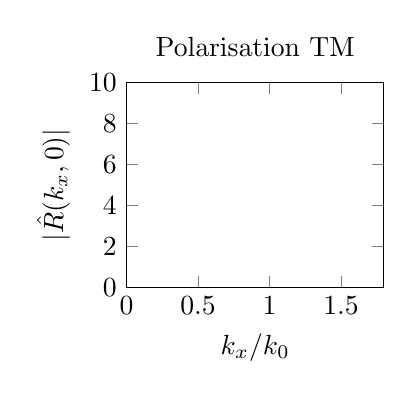
\begin{tikzpicture}[scale=1]
    \begin{axis}[
            title={Polarisation TM},
            ylabel={\(|\hat{R}(k_x,0)|\)},
            xlabel={\(k_x\slash k_0\)},
            width=0.4\textwidth,
            ymin=0,
            ymax=10,
            restrict y to domain=0:+4E+01,
            xmin=0,
            xmax=1.8,
            mark repeat=40,
            legend pos=outer north east
        ]
        % \addplot [color=black,mark=square*] table [col sep=comma, x={s1}, y={Abs(r_ex.tm)}] {csv/SOUDAIS/SOUDAIS.r_ex.MODE_2_TYPE_P.csv};
        % % \addlegendentry{Exact};

        % \addplot [color=blue,mark=x] table [col sep=comma, x={s1}, y={Abs(r_ibc0.tm)}] {csv/SOUDAIS/SOUDAIS.r_ibc.IBC_ibc0_SUC_F_MODE_2_TYPE_P.csv};
        % % \addlegendentry{CI0};

        % \addplot [color=red,mark=diamond*] table [col sep=comma, x={s1}, y={Abs(r_ibc3.tm)}] {csv/SOUDAIS/SOUDAIS.r_ibc.IBC_ibc3_SUC_F_MODE_2_TYPE_P.csv};
        % % \addlegendentry{CI3};
    \end{axis}
\end{tikzpicture}
\tikzsetnextfilename{R_SOUDAIS_plan_hoibc.TE}
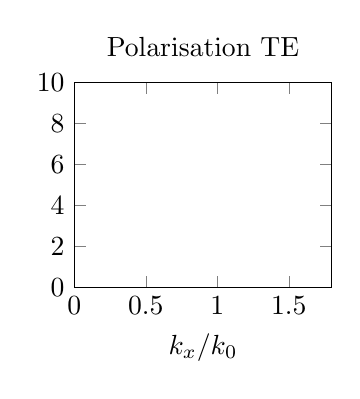
\begin{tikzpicture}[scale=1]
    \begin{axis}[
            title={Polarisation TE},
            ylabel={},
            xlabel={\(k_x\slash k_0\)},
            width=0.4\textwidth,
            xmin=0,
            xmax=1.8,
            ymin=0,
            ymax=10,
            mark repeat=40,
            legend pos=outer north east
        ]
        % \addplot [color=black,mark=square*] table [col sep=comma, x={s1}, y={Abs(r_ex.te)}] {csv/SOUDAIS/SOUDAIS.r_ex.MODE_2_TYPE_P.csv};
        % \addlegendentry{Exact};

        % \addplot [color=blue,mark=x] table [col sep=comma, x={s1}, y={Abs(r_ibc0.te)},color=] {csv/SOUDAIS/SOUDAIS.r_ibc.IBC_ibc0_SUC_F_MODE_2_TYPE_P.csv};
        % \addlegendentry{CI0};

        % \addplot [color=red,mark=diamond*] table [col sep=comma, x={s1}, y={Abs(r_ibc3.te)}] {csv/SOUDAIS/SOUDAIS.r_ibc.IBC_ibc3_SUC_F_MODE_2_TYPE_P.csv};
        % \addlegendentry{CI3};
    \end{axis}
\end{tikzpicture}
          \caption[CIOE sur empilement de P.~Soudais p.~11]{Module des coefficients diagonaux de \(\mR\) pour \(\eps = 4, \mu = 1, d=0.035\text{m}, f=12\text{GHz}\)}
          \label{fig:reflex_fourier:plan:soudais:hoibc}
      \end{figure}

      La figure \ref{fig:imp_fourier:plan:triple_asymptote:hoibc} montre la limite de la CI3 pour capturer 3 asymptotes. Pour cela, il faudrait utiliser une CI d'ordre au moins 6.

      L'expression de cette CIOE que l'on nomme \hyperlink{ci7}{CI7} est
      \begin{equation}
        \left(\oI + \sum_{i=1}^3 \left(d_{i} \left(\frac{\LD}{k_0^2}\right)^i + e_{i} \left(-\frac{\LR}{k_0^2}\right)^i \right)\right)\vE_t = \left(a_0 \oI + \sum_{i=1}^3 \left(b_{i} \left(\frac{\LD}{k_0^2}\right)^i + c_{i} \left(-\frac{\LR}{k_0^2}^i\right) \right)\right)\vJ
      \end{equation}

      \begin{figure}[!hbt]
          \centering
          \tikzsetnextfilename{Z_triple_asymptote_plan_hoibc_TM}
\begin{tikzpicture}[scale=1]
    \begin{axis}[
            title={Polarisation TM},
            ylabel={\(\Im(\hat{Z}(k_x,0)\)},
            xlabel={\(k_x\slash k_0\)},
            width=0.4\textwidth,
            xmin=0,
            xmax=1.999,
            ymin=-10,
            ymax=10,
            restrict y to domain=-300:300,
            mark repeat=200,
            legend pos=outer north east
        ]
        \addplot [color=black,mark=square*] table [col sep=comma, x={s1}, y={Im(z_ex.tm)}] {csv/triple_asymptote/triple_asymptote.z_ex.P.csv};
        % \addlegendentry{Exact};

        \addplot [color=blue,mark=x] table [col sep=comma, x={s1}, y={Im(z_ibc0.tm)}] {csv/triple_asymptote/triple_asymptote.z_ibc.IBC_ibc0_TYPE_P_SUC_F.csv};
        % \addlegendentry{CI0};

        \addplot [color=red,mark=diamond*] table [col sep=comma, x={s1}, y={Im(z_ibc3.tm)}] {csv/triple_asymptote/triple_asymptote.z_ibc.IBC_ibc3_TYPE_P_SUC_F.csv};
        % \addlegendentry{CI3};

        \addplot [color=cyan,mark=pentagon*] table [col sep=comma, x={s1}, y={Im(z_ibc7.tm)}] {csv/triple_asymptote/triple_asymptote.z_ibc.IBC_ibc7_TYPE_P_SUC_F.csv};
        % \addlegendentry{CI7};
    \end{axis}
\end{tikzpicture}
\tikzsetnextfilename{Z_triple_asymptote_plan_hoibc_TE}
\begin{tikzpicture}[scale=1]
    \begin{axis}[
            title={Polarisation TE},
            ylabel={},
            xlabel={\(k_x\slash k_0\)},
            width=0.4\textwidth,
            xmin=0,
            xmax=1.999,
            ymin=-10,
            ymax=10,
            restrict y to domain=-300:300,
            mark repeat=200,
            legend pos=outer north east
        ]
        \addplot [color=black,mark=square*] table [col sep=comma, x={s1}, y={Im(z_ex.te)}] {csv/triple_asymptote/triple_asymptote.z_ex.P.csv};
        \addlegendentry{Exact};

        \addplot [color=blue,mark=x] table [col sep=comma, x={s1}, y={Im(z_ibc0.te)}] {csv/triple_asymptote/triple_asymptote.z_ibc.IBC_ibc0_TYPE_P_SUC_F.csv};
        \addlegendentry{CI0};

        \addplot [color=red,mark=diamond*] table [col sep=comma, x={s1}, y={Im(z_ibc3.te)}] {csv/triple_asymptote/triple_asymptote.z_ibc.IBC_ibc3_TYPE_P_SUC_F.csv};
        \addlegendentry{CI3};

        \addplot [color=cyan,mark=pentagon*] table [col sep=comma, x={s1}, y={Im(z_ibc7.te)}] {csv/triple_asymptote/triple_asymptote.z_ibc.IBC_ibc7_TYPE_P_SUC_F.csv};
        \addlegendentry{CI7};                  
    \end{axis}
\end{tikzpicture}
          \caption[CIOE sur empilement avec triple asymptote]{Partie imaginaire des coefficients diagonaux de \(\mZ\) pour \(\eps = 4, \mu = 1, d=0.2\text{m}, f=1\text{GHz}\)}
          \label{fig:imp_fourier:plan:triple_asymptote:hoibc}
      \end{figure}
      \begin{table}[!hbt]
        \centering
        \begin{minipage}[t]{0.49\textwidth}
        \vspace{0pt}
        \centering
        \begin{coefftable}{\hyperlink{ci0}{CI0}}
          \input{csv/triple_asymptote/triple_asymptote.IBC_ibc0_SUC_F_MODE_2_TYPE_P.coeff.txt}
        \end{coefftable}

        \begin{coefftable}{\hyperlink{ci3}{CI3}}
          \input{csv/triple_asymptote/triple_asymptote.IBC_ibc3_SUC_F_MODE_2_TYPE_P.coeff.txt}
        \end{coefftable}
        \end{minipage}
        \tablecoeff[0.49]{\hyperlink{ci7}{CI7}}{csv/triple_asymptote/triple_asymptote.IBC_ibc7_SUC_F_MODE_2_TYPE_P.coeff.txt}
        \caption{Coefficients associés à la figure \ref{fig:imp_fourier:plan:triple_asymptote:hoibc}}
        \label{tab:imp_fourier:plan:triple_asymptote:hoibc}
      \end{table}
      Il faut donc une CIOE d'ordre 2 fois le nombre d'asymptote que l'on rencontre sur notre balayage.

\subsection{Énoncé de la minimisation au sens des moindres carrés avec contraintes}
  Le problème des moindres carrés avec \gls{acr-csu} s'énonce:

  \begin{prop}[Moindres carrés avec CSU dans le cas plan infini]
  ~

  Soit \(SUC(CI)\) les conditions suffisante d'unicité associées à la CIOE \(CI\). 

  Alors les coefficients de la CIOE sont solution de 

  Trouver \(X_{CI}^*\) tel que

  \[
    X_{CI}^* = \argmin{X \in SUC(CI)} \left\lVert {\mH}(CI)X_{CI} - {b}\right\rVert^2_{\RR^{Ni}}
  \]
  \end{prop}
